\documentclass[11pt,a4paper]{article}

% Packages
\usepackage[utf8]{inputenc}
\usepackage[T1]{fontenc}
\usepackage{amsmath,amssymb,amsthm,mathtools}
\usepackage{graphicx}
\usepackage{booktabs}
\usepackage{siunitx}
\usepackage{xcolor}
\usepackage{hyperref}
\usepackage[margin=1in]{geometry}
\usepackage{float}
\usepackage{caption}
\usepackage{subcaption}
\usepackage{enumitem}
\usepackage{tikz}
\usepackage{tcolorbox}
\usetikzlibrary{arrows.meta,positioning,shapes,decorations.pathreplacing}

% Custom commands
\newcommand{\kfold}{k_{\text{fold}}}
\newcommand{\kon}{k_{\text{on}}}
\newcommand{\koff}{k_{\text{off}}}
\newcommand{\kelong}{k_{\text{elong}}}
\newcommand{\kinit}{k_{\text{init}}}
\newcommand{\Ttotal}{T_{\text{total}}}
\newcommand{\temerge}{t_{\text{emerge}}}
\newcommand{\taufold}{\tau_{\text{fold}}}
\newcommand{\tauon}{\tau_{\text{on}}}
\newcommand{\tauoff}{\tau_{\text{off}}}

\title{\textbf{Modeling Co-Translational Protein Folding}}
\author{Luis U. Aguilera}
\date{\today}

\begin{document}

\maketitle

\begin{abstract}
We develop kinetic models to explain co-translational protein folding as measured by the coTFT (Co-Translational Folding Tracking) technology. The experimental system uses tandem GFP domains fused to an smHA tag, where folding is detected by intrabody binding to folded GFP. A key observation is that co-translational folding efficiency increases from 40\% (1$\times$GFP) to 67\% (6$\times$GFP), plateauing at $\sim$3--4 copies. We test the \textbf{time constraint hypothesis}: later-synthesized domains have insufficient time to fold before translation terminates. We compare two models: (1) a \textbf{One-Pool model} (1 parameter) assuming all nascent chains can fold, and (2) a \textbf{Two-Pool model} (3 parameters) assuming nascent chains comprise two populations: one capable of folding and one that is not. The One-Pool model fails, predicting decreasing efficiency. The Two-Pool model successfully reproduces the data with $\kfold = 0.013$ s$^{-1}$ ($\taufold \approx 78$s), a baseline foldable fraction $f_{\text{base}} = 42\%$, and an avidity gain of $f_{\text{gain}} = 12\%$ per additional domain. The biological implications suggest that nascent chain populations are inherently heterogeneous, with only $\sim$42\% capable of productively folding during translation. Adding more GFP domains provides additional ``chances'' for successful folding, explaining the saturation behavior at 3--4 copies.
\end{abstract}

% Table of contents removed for cleaner document
\vspace{1em}

%==============================================================================
\section{Experimental System Overview}
%==============================================================================

The Co-Translational Folding Tracking (coTFT) system enables real-time visualization of protein folding during translation using dual-color single-molecule microscopy. The reporter mRNA encodes (N- to C-terminus): an \textbf{smHA tag} with 10$\times$ HA epitopes, up to 6$\times$ \textbf{tandem ``dark'' GFP domains}, and \textbf{MS2 stem loops} for mRNA visualization, giving a total protein length of $L_{\text{total}} = 1826$ amino acids. Two fluorescent probes enable simultaneous detection: nascent chain emergence via an anti-HA intrabody fused to HaloTag-JF646, and protein folding via the anti-GFP intrabody LaG16 fused to mStayGold, which binds only to properly folded GFP $\beta$-barrel structures. The ``dark'' GFP mutations eliminate intrinsic fluorescence while preserving native folding. Seven constructs were tested with varying numbers of GFP vs.\ mCherry (non-folding control) domains. GFP domains are always positioned at the N-terminus (synthesized first), followed by mCherry domains at the C-terminus.


%==============================================================================
\section{Experimental Data}
%==============================================================================

Co-translational folding (CoF) efficiency is measured using single-molecule microscopy and colocalization analysis. Individual translation sites (polysomes) are first identified in the nascent chain channel via anti-HA intrabody binding to the smHA tag, where each spot represents a single mRNA being actively translated, typically carrying multiple ribosomes. For each polysome spot, we then determine whether there is a colocalized spot in the folding channel, indicating anti-GFP intrabody binding to folded GFP domains on nascent chains. CoF efficiency is calculated as the fraction of spots that show colocalized folding signal:

\begin{equation}
\text{CoF Efficiency} = \frac{\text{Number of spots with folding signal}}{\text{Total number of spots}} \times 100\%
\end{equation}

\begin{table}[H]
\centering
\caption{Experimental CoF efficiency measurements}
\label{tab:exp_data}
\begin{tabular}{@{}cccc@{}}
\toprule
\textbf{$n_{\text{GFP}}$} & \textbf{Mean (\%)}& \textbf{SEM (\%)} & \textbf{$N$ (cells)} \\
\midrule
0 & 2.3 & 0.2 & 15 \\
1 & 40.0 & 2.4 & 17 \\
2 & 49.8 & 2.5 & 20 \\
3 & 62.1 & 2.4 & 19 \\
4 & 66.7 & 1.8 & 20 \\
5 & 65.6 & 1.8 & 19 \\
6 & 66.6 & 1.8 & 16 \\
\bottomrule
\end{tabular}
\end{table}

The data reveal a characteristic saturation behavior: CoF efficiency increases from 40\% (1$\times$GFP) to $\sim$66\% (4$\times$GFP), then plateaus at $\sim$66\% for constructs with 4--6 GFP domains. The 6$\times$mCherry control shows only $\sim$2.3\% (non-specific colocalization). At 67\% efficiency with 6 GFP domains, approximately $6 \times 0.67 \approx 4$ copies are detected as folded on average, suggesting a physical limit on the number of detectable domains.

%==============================================================================
\section{Physical Parameters and Time Windows}
%==============================================================================

We used autocorrelation analysis to estimate translation kinetics from our single-molecule data. The key parameters are the elongation rate $\kelong = 4.85$ aa/s and initiation rate $\kinit = 0.063$ ribosomes/s. The initiation rate provides context about the polysome environment: mean ribosome spacing is $\kelong / \kinit = 4.85 / 0.063 = 77$ aa, with approximately $L_{\text{total}} / 77 \approx 24$ ribosomes per mRNA on average. Since ribosomes are spaced 77 aa apart (much greater than the $\sim$10 aa ribosome footprint), each nascent chain folds independently without interference from neighboring ribosomes. Taking initiation and elongation rates, together with the construct architecture, determine the time available for each domain to fold. The total translation time for the 1826 aa construct is:
\begin{equation}
\Ttotal = \frac{L_{\text{total}}}{\kelong} = \frac{1826 \text{ aa}}{4.85 \text{ aa/s}} = 377 \text{ s} \approx 6.3 \text{ min}
\end{equation}

Each GFP domain emerges from the ribosome exit tunnel at time $\temerge^{(i)}$, leaving a time window $\Delta t_i = \Ttotal - \temerge^{(i)}$ for folding before translation terminates:

\begin{table}[H]
\centering
\caption{GFP domain positions, emergence times, and available time windows}
\label{tab:emergence}
\begin{tabular}{@{}ccccc@{}}
\toprule
\textbf{Domain} & \textbf{C-terminus (aa)} & \textbf{Exit tunnel (aa)$^*$} & $\temerge^{(i)}$ \textbf{(s)} & \textbf{Time window (s)} \\
\midrule
GFP$_1$ & 590 & 625 & 129 & 248 \\
GFP$_2$ & 835 & 870 & 179 & 197 \\
GFP$_3$ & 1080 & 1115 & 230 & 147 \\
GFP$_4$ & 1325 & 1360 & 280 & 96 \\
GFP$_5$ & 1570 & 1605 & 331 & 46 \\
GFP$_6$ & 1815 & 1826$^\dagger$ & 376 & 0 \\
\bottomrule
\end{tabular}

\vspace{0.3em}
\parbox{0.95\textwidth}{\footnotesize
$^*$Exit tunnel position = C-terminus + 35 aa (ribosome exit tunnel length). \\
$^\dagger$For GFP$_6$, the exit tunnel position is capped at the construct end (1826 aa), since 1815 + 35 = 1850 aa exceeds the total construct length.
}
\end{table}

Figure~\ref{fig:timeline} visualizes the translation timeline, showing when each GFP domain emerges and the time remaining for folding.

\begin{figure}[H]
\centering
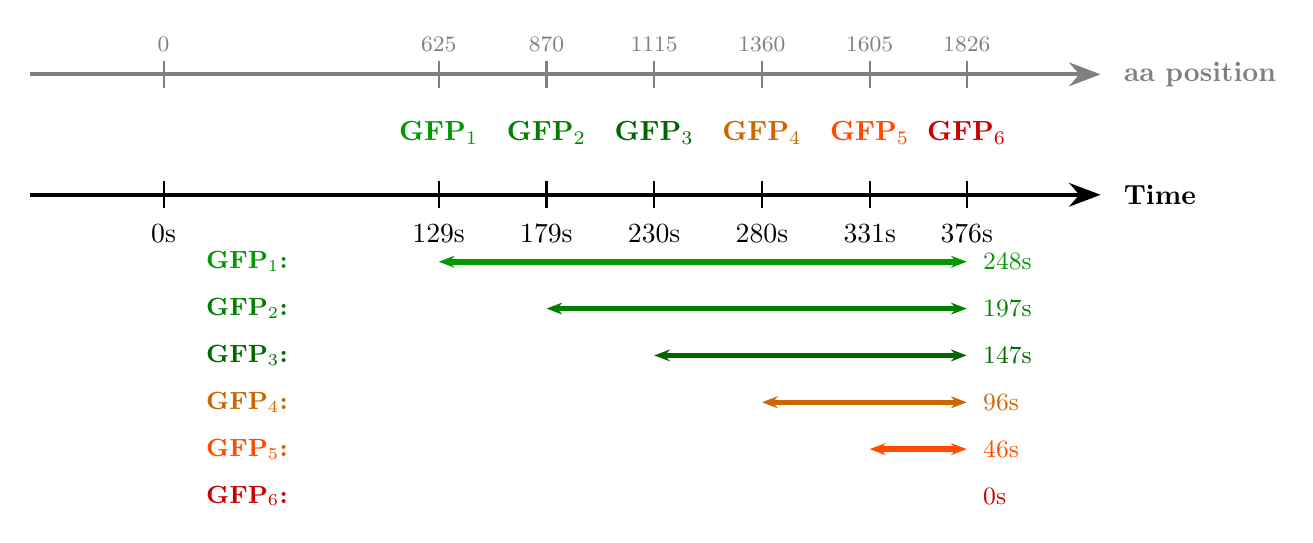
\begin{tikzpicture}[scale=0.85]
    % Amino acid position ruler (top)
    \draw[-{Stealth[length=4mm]}, line width=1.5pt, gray] (0,1.8) -- (16,1.8);
    \node[right, gray] at (16.2,1.8) {\textbf{aa position}};
    
    % AA tick marks - positions where domain C-terminus clears tunnel
    % New scale: x = 2 + (aa/1826) * 12 to compress left and spread right
    % Emergence positions from GFP_positions.csv: 625, 870, 1115, 1360, 1605, 1826
    \draw[thick, gray] (2, 2.0) -- (2, 1.6);
    \node[above, gray, font=\footnotesize] at (2, 2.0) {0};
    
    \draw[thick, gray] (6.11, 2.0) -- (6.11, 1.6);
    \node[above, gray, font=\footnotesize] at (6.11, 2.0) {625};
    
    \draw[thick, gray] (7.72, 2.0) -- (7.72, 1.6);
    \node[above, gray, font=\footnotesize] at (7.72, 2.0) {870};
    
    \draw[thick, gray] (9.33, 2.0) -- (9.33, 1.6);
    \node[above, gray, font=\footnotesize] at (9.33, 2.0) {1115};
    
    \draw[thick, gray] (10.94, 2.0) -- (10.94, 1.6);
    \node[above, gray, font=\footnotesize] at (10.94, 2.0) {1360};
    
    \draw[thick, gray] (12.55, 2.0) -- (12.55, 1.6);
    \node[above, gray, font=\footnotesize] at (12.55, 2.0) {1605};
    
    \draw[thick, gray] (14, 2.0) -- (14, 1.6);
    \node[above, gray, font=\footnotesize] at (14, 2.0) {1826};

    % Main timeline arrow (time)
    \draw[-{Stealth[length=4mm]}, line width=1.5pt] (0,0) -- (16,0);
    \node[right] at (16.2,0) {\textbf{Time}};
    
    % Time tick marks and labels
    % Emergence times: 129s, 179s, 230s, 280s, 331s, 376s
    % x = 2 + (t/376.5) * 12
    \draw[thick] (2, 0.2) -- (2, -0.2);
    \node[below] at (2, -0.3) {0s};
    
    \draw[thick] (6.11, 0.2) -- (6.11, -0.2);
    \node[below] at (6.11, -0.3) {129s};
    \node[above, green!60!black, font=\bfseries] at (6.11, 0.6) {GFP$_1$};
    
    \draw[thick] (7.72, 0.2) -- (7.72, -0.2);
    \node[below] at (7.72, -0.3) {179s};
    \node[above, green!50!black, font=\bfseries] at (7.72, 0.6) {GFP$_2$};
    
    \draw[thick] (9.33, 0.2) -- (9.33, -0.2);
    \node[below] at (9.33, -0.3) {230s};
    \node[above, green!40!black, font=\bfseries] at (9.33, 0.6) {GFP$_3$};
    
    \draw[thick] (10.94, 0.2) -- (10.94, -0.2);
    \node[below] at (10.94, -0.3) {280s};
    \node[above, orange!80!black, font=\bfseries] at (10.94, 0.6) {GFP$_4$};
    
    \draw[thick] (12.55, 0.2) -- (12.55, -0.2);
    \node[below] at (12.55, -0.3) {331s};
    \node[above, orange!60!red, font=\bfseries] at (12.55, 0.6) {GFP$_5$};
    
    \draw[thick] (14, 0.2) -- (14, -0.2);
    \node[below] at (14, -0.3) {376s};
    \node[above, red!80!black, font=\bfseries] at (14, 0.6) {GFP$_6$};
    
    % Time window bars (stacked below, with labels on left)
    % Time windows from model: 248s, 197s, 147s, 96s, 46s, 0s
    \node[left, green!60!black, font=\small\bfseries] at (4, -1.0) {GFP$_1$:};
    \draw[{Stealth[length=2mm]}-{Stealth[length=2mm]}, line width=2pt, green!60!black] 
        (6.11, -1.0) -- (14, -1.0);
    \node[right, green!60!black, font=\small] at (14.1, -1.0) {248s};
    
    \node[left, green!50!black, font=\small\bfseries] at (4, -1.7) {GFP$_2$:};
    \draw[{Stealth[length=2mm]}-{Stealth[length=2mm]}, line width=2pt, green!50!black] 
        (7.72, -1.7) -- (14, -1.7);
    \node[right, green!50!black, font=\small] at (14.1, -1.7) {197s};
    
    \node[left, green!40!black, font=\small\bfseries] at (4, -2.4) {GFP$_3$:};
    \draw[{Stealth[length=2mm]}-{Stealth[length=2mm]}, line width=2pt, green!40!black] 
        (9.33, -2.4) -- (14, -2.4);
    \node[right, green!40!black, font=\small] at (14.1, -2.4) {147s};
    
    \node[left, orange!80!black, font=\small\bfseries] at (4, -3.1) {GFP$_4$:};
    \draw[{Stealth[length=2mm]}-{Stealth[length=2mm]}, line width=2pt, orange!80!black] 
        (10.94, -3.1) -- (14, -3.1);
    \node[right, orange!80!black, font=\small] at (14.1, -3.1) {96s};
    
    \node[left, orange!60!red, font=\small\bfseries] at (4, -3.8) {GFP$_5$:};
    \draw[{Stealth[length=2mm]}-{Stealth[length=2mm]}, line width=2pt, orange!60!red] 
        (12.55, -3.8) -- (14, -3.8);
    \node[right, orange!60!red, font=\small] at (14.1, -3.8) {46s};
    
    \node[left, red!80!black, font=\small\bfseries] at (4, -4.5) {GFP$_6$:};
    \node[right, red!80!black, font=\small] at (14.1, -4.5) {0s};
    
\end{tikzpicture}

\caption{\textbf{Translation timeline for a 6$\times$GFP construct.} Top axis: amino acid position where each domain's C-terminus clears the ribosome exit tunnel (C-terminus + 35 aa, except GFP$_6$ which is capped at construct end). Bottom axis: corresponding emergence time ($t = \text{aa}/k_{\text{elong}}$). Colored bars show the time window $\Delta t_i$ available for each domain to fold before translation terminates at 376 s. Later domains have progressively shorter time windows.}
\label{fig:timeline}
\end{figure}


%==============================================================================
\section{The Time Constraint Hypothesis}
%==============================================================================

The time constraint hypothesis posits that the observed saturation in folding signal arises because later-synthesized domains have progressively shorter time windows to complete folding before translation terminates and the polysome disassembles. For a domain to contribute to the folding signal, it must first emerge from the ribosome exit tunnel and then fold into the native $\beta$-barrel structure (characteristic time $\taufold$) so that the LaG16 intrabody can bind. If $\taufold$ exceeds the available time window $\Delta t_i$, the domain will not be detected. This creates a kinetic competition between folding and translation termination that becomes increasingly severe for later domains.

%==============================================================================
\section{Kinetic Model}
%==============================================================================

\textbf{Irreversible Single-Step Kinetics.} For each GFP domain $i$, we define two state fractions: $U_i(t)$ (\textbf{unfolded}) and $F_i(t)$ (\textbf{folded}). Once folded, the domain can be detected by the LaG16 intrabody, which binds rapidly to the folded GFP $\beta$-barrel structure. The kinetic scheme is:

\begin{center}
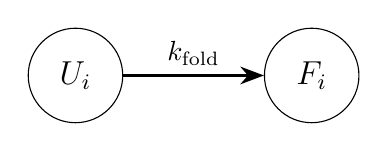
\begin{tikzpicture}[
    node distance=3cm,
    state/.style={circle, draw, minimum size=1.2cm, font=\large},
    arrow/.style={-{Stealth[length=3mm]}, thick}
]
    \node[state] (U) {$U_i$};
    \node[state, right of=U] (F) {$F_i$};
    
    \draw[arrow] (U) -- node[above] {$\kfold$} (F);
\end{tikzpicture}
\end{center}

\noindent The corresponding ODE system is:

\begin{align}
\frac{dU_i}{dt} &= -\kfold \, U_i \\[0.5em]
\frac{dF_i}{dt} &= \kfold \, U_i
\end{align}

\noindent This system has a closed-form solution. For $t \geq 0$ (time since emergence):

\begin{equation}
U_i(t) = e^{-\kfold t}
\end{equation}
Since $U_i(t) + F_i(t) = 1$ (conservation of probability), the folded fraction is:
\begin{equation}
F_i(t) = 1 - U_i(t) = 1 - e^{-\kfold t} \label{eq:folded_fraction}
\end{equation}

\noindent At steady state ($t \to \infty$), the folded fraction approaches unity ($F_i^{ss} = 1$). However, translation terminates before steady state is reached. The key quantity for modeling CoF efficiency is the folded fraction at termination:
\begin{equation}
F_i(\Delta t_i) = 1 - e^{-\kfold \cdot \Delta t_i} \label{eq:folded_termination}
\end{equation}
where $\Delta t_i$ is the time window available for domain $i$ to fold before translation terminates.

The ODE solution above describes folding for a single GFP domain. However, our experimental constructs contain between one and six GFP domains. To bridge this gap between single-domain kinetics and construct-level predictions, we implemented a framework that accomplishes three things. First, we calculate $F(\Delta t_i)$ for each domain position $i$ using Eq.~\ref{eq:folded_termination}. Second, we aggregate these individual folded fractions into a single predicted efficiency for each construct (Eq.~\ref{eq:onepool_efficiency} and~\ref{eq:twopool_efficiency}). Third, we fit the kinetic parameters across all constructs by comparing six model predictions to their corresponding experimental means using weighted least-squares optimization (Section~\ref{sec:parameter_estimation}). 

With this framework established, we now develop two alternative models that make different assumptions about which nascent chains can fold. The \textbf{One-Pool model} (Section~\ref{sec:onepool}) assumes all chains are equally competent for folding, serving as a kinetic null hypothesis. The \textbf{Two-Pool model} (Section~\ref{sec:twopool}) introduces population heterogeneity, allowing for the possibility that only a fraction of chains can fold co-translationally.

%==============================================================================
\section{The One-Pool Model (Pure Kinetic)}
\label{sec:onepool}
%==============================================================================

The One-Pool model assumes that 100\% of nascent chains can fold. The only factors determining CoF efficiency are the folding rate and the available time windows:
\begin{equation}
\text{CoF Efficiency}(n_{\text{GFP}}) = \frac{100}{n_{\text{GFP}}} \sum_{i=1}^{n_{\text{GFP}}} F(\Delta t_i; \kfold)
\label{eq:onepool_efficiency}
\end{equation}
where $n_{\text{GFP}}$ is the number of GFP domains in the construct (1--6), $i$ indexes each domain position, and $F(\Delta t_i)$ is the folded fraction for domain $i$ given its available time window $\Delta t_i$ before translation terminates. This model has 1 free parameter: $\kfold$.

Using the optimization method described in Section~\ref{sec:parameter_estimation}, the best-fit One-Pool model parameters are:

\begin{table}[H]
\centering
\caption{Fitted parameters for the One-Pool model}
\label{tab:onepool_params}
\begin{tabular}{@{}llll@{}}
\toprule
\textbf{Parameter} & \textbf{Value} & \textbf{Units} & \textbf{Interpretation} \\
\midrule
$\kfold$ & 0.0057 & s$^{-1}$ & GFP folding rate ($\taufold = 175$ s) \\
\bottomrule
\end{tabular}
\end{table}

Observing Fig. \ref{fig:onepool_solution}, the One-Pool model fails as it predicts efficiency should decrease while the data shows an increase (40\% $\to$ 67\%).

\begin{tcolorbox}[colback=gray!10, colframe=gray!50, arc=2mm, boxrule=0.5pt]
\textbf{Worked Example (3$\times$GFP):} Using the fitted $\kfold = 0.0057$ s$^{-1}$ ($\taufold = 175$s) and time windows from Table~\ref{tab:emergence}: $\Delta t_1 = 248$s, $\Delta t_2 = 197$s, $\Delta t_3 = 147$s. The folded fractions are:
\begin{align*}
F(\Delta t_1) &= 1 - e^{-0.0057 \times 248} = 0.76 \quad (76\%) \\
F(\Delta t_2) &= 1 - e^{-0.0057 \times 197} = 0.68 \quad (68\%) \\
F(\Delta t_3) &= 1 - e^{-0.0057 \times 147} = 0.57 \quad (57\%)
\end{align*}
Applying Eq.~\ref{eq:onepool_efficiency}: $\text{CoF}(3) = \frac{100}{3}(0.76 + 0.68 + 0.57) = 67\%$. The experimental value is 62\%, but critically, the model predicts higher efficiency for 1$\times$GFP (76\%) than for 3$\times$GFP (67\%).
\end{tcolorbox}

\begin{figure}[H]
\centering
\includegraphics[width=0.95\textwidth]{../modeling/figures/fig2_onepool_solution.png}
\caption{\textbf{One-Pool Model: Pure Kinetics Fails.} 
(A) Model fit shows the One-Pool model predicts decreasing efficiency with more domains, opposite to the experimental trend.
(B) Schematic of the One-Pool model assuming all nascent chains are competent for folding.
(C) Fitted parameter: $\kfold = 0.0057$ s$^{-1}$ ($\taufold = 175$ s).
(D) Translation timeline showing the time windows for folding for each GFP domain.}
\label{fig:onepool_solution}
\end{figure}

\begin{figure}[H]
\centering
\includegraphics[width=0.3\textwidth]{../modeling/figures/fig3_onepool_parameters.png}
\caption{\textbf{One-Pool Model: Parameter Sensitivity.} 
Sensitivity of $\chi^2$ (weighted MSE) to $\tau_{\text{fold}}$ (30--250s). The dotted line marks the best-fit $\tau_{\text{fold}} = 175$s that minimizes $\chi^2$. }
\label{fig:onepool_params}
\end{figure}

%==============================================================================
\section{The Two-Pool Model}
\label{sec:twopool}
%==============================================================================

\textbf{The Two-Pool Hypothesis.} Not all nascent chains may be competent for co-translational folding. We propose two populations: (1) chains that can productively fold, and (2) chains that cannot fold efficiently due to misfolding, aggregation, or kinetic traps. The key insight is that the effective fraction of foldable chains, $f_{\text{eff}}$, increases with more GFP domains. That is having more domains provides more opportunities to ``catch'' at least one properly folded domain (an avidity effect). We model this as:
\begin{align}
f_{\text{eff}}(n_{\text{GFP}}) &= \min\left(1, f_{\text{base}} + f_{\text{gain}} \cdot (n_{\text{GFP}} - 1)\right) \\[0.5em]
\text{CoF Efficiency}(n_{\text{GFP}}) &= f_{\text{eff}}(n_{\text{GFP}}) \cdot \frac{100}{n_{\text{GFP}}} \sum_{i=1}^{n_{\text{GFP}}} F(\Delta t_i; \kfold) \label{eq:twopool_efficiency}
\end{align}

The parameter $f_{\text{base}}$ is the baseline foldable fraction when only one GFP domain is present. The parameter $f_{\text{gain}}$ is the additional foldable fraction gained per extra GFP domain. Together, these define $f_{\text{eff}}(n_{\text{GFP}})$, which increases linearly with the number of domains until reaching 100\%.

\subsection{Best-Fit Model: Two-Pool Results}

The fitted parameters and their physical interpretation are summarized in Table~\ref{tab:twopool_params}.

\begin{table}[H]
\centering
\caption{Fitted parameters for the Two-Pool model}
\label{tab:twopool_params}
\begin{tabular}{@{}llll@{}}
\toprule
\textbf{Parameter} & \textbf{Value} & \textbf{Units} & \textbf{Interpretation} \\
\midrule
$\kfold$ & 0.013 & s$^{-1}$ & GFP folding rate ($\taufold = 78$ s) \\
$f_{\text{base}}$ & 0.42 & --- & Baseline foldable fraction (42\%) \\
$f_{\text{gain}}$ & 0.12 & per domain & Increase per additional GFP \\
\bottomrule
\end{tabular}
\end{table}

\begin{tcolorbox}[colback=gray!10, colframe=gray!50, arc=2mm, boxrule=0.5pt]
\textbf{Worked Example (3$\times$GFP):} Using fitted parameters $\kfold = 0.013$ s$^{-1}$, $f_{\text{base}} = 0.42$, and $f_{\text{gain}} = 0.12$. First, calculate the effective foldable fraction:
\[
f_{\text{eff}}(3) = \min(1, 0.42 + 0.12 \times (3-1)) = \min(1, 0.66) = 0.66 \quad (66\%)
\]
Next, calculate folded fractions using Eq.~\ref{eq:folded_termination} with time windows $\Delta t_1 = 248$s, $\Delta t_2 = 197$s, $\Delta t_3 = 147$s:
\begin{align*}
F(\Delta t_1) &= 1 - e^{-0.013 \times 248} = 0.96 \quad (96\%) \\
F(\Delta t_2) &= 1 - e^{-0.013 \times 197} = 0.92 \quad (92\%) \\
F(\Delta t_3) &= 1 - e^{-0.013 \times 147} = 0.85 \quad (85\%)
\end{align*}
Applying Eq.~\ref{eq:twopool_efficiency}: $\text{CoF}(3) = 0.66 \times \frac{100}{3}(0.96 + 0.92 + 0.85) = 0.66 \times 91\% = 60\%$. This closely matches the experimental value of 62\%.
\end{tcolorbox}

\begin{figure}[H]
\centering
\includegraphics[width=0.85\textwidth]{../modeling/figures/fig4_twopool_solution.png}
\caption{\textbf{Two-Pool Model:} 
(A) Model fit shows agreement with experimental data, correctly predicting the increasing efficiency trend.
(B) Schematic of the Two-Pool model with foldable and non-foldable populations.
(C) Fitted parameters: $\kfold = 0.013$ s$^{-1}$ ($\taufold = 78$ s), $f_{\text{base}} = 0.42$, $f_{\text{gain}} = 0.12$.
(D) Translation timeline showing the time windows for folding for each GFP domain.}
\label{fig:twopool_solution}
\end{figure}

\begin{figure}[H]
\centering
\includegraphics[width=0.8\textwidth]{../modeling/figures/fig5_twopool_parameter_space.png}
\caption{\textbf{Two-Pool Model: Parameter Space Analysis.} 
Pairwise 2D sweeps showing $\chi^2$ (weighted MSE) as a function of parameter pairs (other parameters held at best-fit values). Dark regions indicate better fits (lower $\chi^2$); red stars indicate best-fit values that minimize $\chi^2$.
(A) $\taufold$ ($= 1/\kfold$) vs $f_{\text{base}}$. (B) $\taufold$ ($= 1/\kfold$) vs $f_{\text{gain}}$. (C) $f_{\text{base}}$ vs $f_{\text{gain}}$.}
\label{fig:twopool_space}
\end{figure}

\begin{figure}[H]
\centering
\includegraphics[width=0.8\textwidth]{../modeling/figures/fig6_twopool_sensitivity.png}
\caption{\textbf{Two-Pool Model: Parameter Sensitivity.} 
Sensitivity of $\chi^2$ (weighted MSE) to each parameter while holding other parameters at best-fit values. Shaded regions indicate acceptable ranges ($\chi^2 \leq 2\times$ best); dashed lines mark best-fit values.
(A) $\tau_{\text{fold}}$ sensitivity. 
(B) $f_{\text{base}}$ sensitivity. 
(C) $f_{\text{gain}}$ sensitivity.}
\label{fig:sensitivity}
\end{figure}


%==============================================================================
\section{Parameter Estimation}
\label{sec:parameter_estimation}
%==============================================================================

Parameters are estimated by minimizing the weighted sum of squared residuals (chi-squared):
\begin{equation}
\chi^2 = \sum_{n_{\text{GFP}}=1}^{6} \left( \frac{\text{CoF}_{\text{model}}(n_{\text{GFP}}) - \text{CoF}_{\text{exp}}(n_{\text{GFP}})}{\text{SEM}_{n_{\text{GFP}}}} \right)^2
\end{equation}

We use differential evolution, a global optimization algorithm suitable for non-convex objective functions with multiple local minima, followed by L-BFGS-B local refinement. The parameter bounds used during optimization are:
\begin{itemize}
\item $\kfold \in [0.004, 0.033]$ s$^{-1}$: GFP folding rate ($\taufold \in [30, 250]$ s)
\item $f_{\text{base}} \in [0.2, 0.8]$: Baseline foldable fraction (Two-Pool model only)
\item $f_{\text{gain}} \in [0.01, 0.2]$: Gain per additional GFP domain (Two-Pool model only)
\end{itemize}

%==============================================================================
\section{Conclusions}
%==============================================================================

The Two-Pool model explains the saturation behavior by proposing that only $\sim$42\% of nascent chains are initially competent for co-translational folding, with each additional GFP domain increasing this fraction by $\sim$12\% (avidity effect). The fitted folding rate $\kfold = 0.013$ s$^{-1}$ ($\taufold \approx 78$s) is consistent with in vitro GFP folding kinetics. The time constraint hypothesis explains why later GFP domains contribute less to the signal: they have progressively shorter time windows before translation terminates and the polysome disassembles, leaving insufficient time to complete the folding process.

\textbf{Simplifying assumptions.} Translation termination is modeled as instantaneous at the stop codon, and only folding completed before ribosome release contributes to the measured signal. All GFP domains are assumed to fold with identical rate constants ($\kfold$), and intrabody binding to folded GFP is assumed to be fast relative to folding (not rate-limiting). The model uses time-averaged polysome parameters rather than stochastic simulation of individual ribosome dynamics.

%==============================================================================
\end{document}

